\documentclass[tikz,border=6pt]{standalone}
\usepackage{amsmath,amssymb}
\usepackage{tikz}
\usetikzlibrary{calc,arrows.meta,positioning}

\tikzset{
	axis/.style={thick,->,>=Stealth},
	vec/.style={thick,->,>=Stealth},
	aux/.style={thin,dashed},
	err/.style={blue!70!black,thick,->,>=Stealth},
	mainline/.style={thick},
	pt/.style={circle,fill=black,inner sep=1.2pt},
	usvfill/.style={fill=gray!35},
	usvdraw/.style={thick},
	usvcenterline/.style={thin}
}

% -------------------------------------------------
% USV: hull + body-fixed frame
% usage: \drawusvframe{(shift)}{rotation angle}{scale}
% -------------------------------------------------
\newcommand{\drawusvframe}[3]{%
	\begin{scope}[shift={#1}, rotate=#2, scale=#3]
		% hull
		\path[usvfill]
		(0,1.15)
		.. controls (0.28,0.95) and (0.42,0.45) .. (0.40,-0.10)
		.. controls (0.38,-0.48) and (0.30,-0.78) .. (0.24,-0.90)
		-- (-0.24,-0.90)
		.. controls (-0.30,-0.78) and (-0.38,-0.48) .. (-0.40,-0.10)
		.. controls (-0.42,0.45) and (-0.28,0.95) .. cycle;
		
		\draw[usvdraw]
		(0,1.15)
		.. controls (0.28,0.95) and (0.42,0.45) .. (0.40,-0.10)
		.. controls (0.38,-0.48) and (0.30,-0.78) .. (0.24,-0.90)
		-- (-0.24,-0.90)
		.. controls (-0.30,-0.78) and (-0.38,-0.48) .. (-0.40,-0.10)
		.. controls (-0.42,0.45) and (-0.28,0.95) .. cycle;
		
		% centerline
		\draw[usvcenterline] (0,0.92) -- (0,-0.74);
		
		% origin
		\fill (0,0) circle (0.5pt);
		
		% body-fixed frame: x_b forward, y_b right
		\draw[vec] (0,0) -- (0,1.05) node[left] {$x_b$};
		\draw[vec] (0,0) -- (1.00,0) node[above] {$y_b$};
	\end{scope}%
}

\begin{document}
	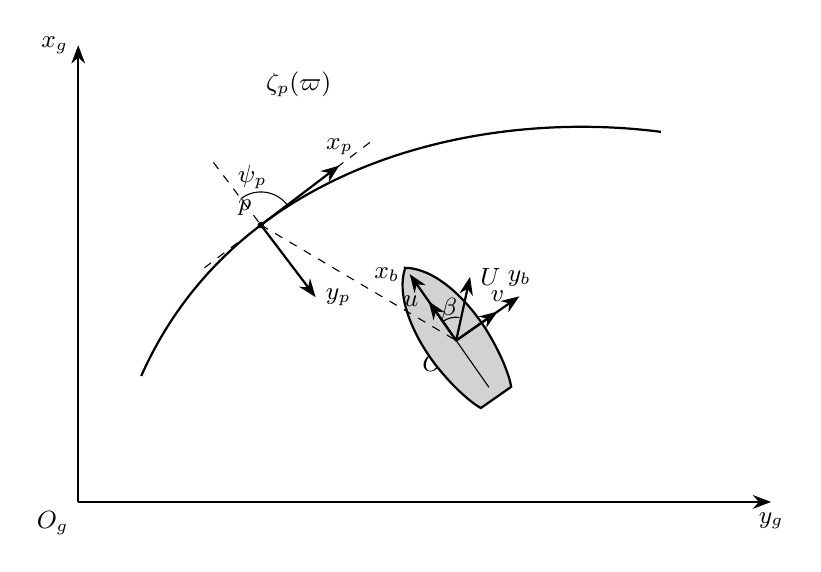
\begin{tikzpicture}[every node/.style={font=\small}]
		
		% -------------------------------------------------
		% 1. Global frame
		% -------------------------------------------------
		\coordinate (Og) at (0,0);
		\draw[axis] (Og) -- (0,5.8) node[left] {$x_g$};
		\draw[axis] (Og) -- (8.8,0) node[below] {$y_g$};
		\node[below left] at (Og) {$O_g$};
		
		% -------------------------------------------------
		% 2. Reference path
		% -------------------------------------------------
		\draw[mainline]
		(0.8,1.6) .. controls (2.0,4.3) and (5.1,5.0) .. (7.4,4.7);
		\node at (2.8,5.3) {$\zeta_p(\varpi)$};
		
		% -------------------------------------------------
		% 3. Reference point on path + local frame
		% -------------------------------------------------
		% Take three nearby points on the same curve
		\path
		(0.8,1.6) .. controls (2.0,4.3) and (5.1,5.0) .. (7.4,4.7)
		coordinate[pos=0.300] (P)
		coordinate[pos=0.292] (Pa)
		coordinate[pos=0.308] (Pb);
		
		% Compute tangent angle from Pa to Pb
		\pgfmathanglebetweenpoints{\pgfpointanchor{Pa}{center}}{\pgfpointanchor{Pb}{center}}
		\let\tangentangle\pgfmathresult
		
		% Draw local frame at p in a rotated scope
		\begin{scope}[shift={(P)}, rotate=\tangentangle]
			\fill (0,0) circle (1.2pt);
			\node[above left] at (0,0) {$p$};
			
			% tangent axis
			\draw[vec] (0,0) -- (1.25,0) node[above] {$x_p$};
			
			% normal axis
			\draw[vec] (0,0) -- (0,-1.15) node[right] {$y_p$};
			
			% auxiliary dashed lines
			\draw[aux] (-0.9,0) -- (1.8,0);
			\draw[aux] (0,1.0) -- (0,-1.1);
			
			% path heading angle
			\draw (0,0.42) arc[start angle=90,end angle=0,radius=0.42];
			\node at (0.28,0.55) {$\psi_p$};
		\end{scope}
		
		% -------------------------------------------------
		% 4. Vessel center and USV
		% -------------------------------------------------
		\coordinate (O) at (4.8,2.05);
		\node[pt,label=below left:$O$] at (O) {};
		\drawusvframe{(O)}{35}{0.98}
		
		% -------------------------------------------------
		% 5. Heading auxiliary lines and psi
		% -------------------------------------------------
%		\draw[aux] ($(O)+(-1.1,-0.32)$) -- ($(O)+(2.0,0.80)$);
%		\draw[aux] ($(O)+(0,1.35)$) -- ($(O)+(0,-1.45)$);
%		
%		\draw ($(O)+(0,0.48)$) arc[start angle=90,end angle=35,radius=0.48];
%		\node at ($(O)+(0.32,0.72)$) {$\psi$};
		
		% -------------------------------------------------
		% 6. Geometric relations
		% -------------------------------------------------
		\draw[aux] (P) -- (O);
		
%		\draw[err] ($(P)+(-0.10,-0.08)$) -- ($(O)+(-0.18,0.08)$)
%		node[midway,left] {$\varepsilon_e$};
%		
%		\draw[err] ($(P)+(0.18,-0.10)$) -- ++(0.48,0)
%		node[midway,below] {$\varepsilon_s$};
%		
%		\draw[aux] ($(O)+(-0.55,-1.20)$) -- ($(P)+(0.18,-0.25)$);
%		\node at (4.02,1.08) {$\xi$};
		
		% -------------------------------------------------
		% 7. Velocity components near vessel
		% -------------------------------------------------
		\begin{scope}[shift={(O)}, rotate=35, scale=0.78]
			\draw[vec] (0,0) -- (0,0.78) node[left] {$u$};
			\draw[vec] (0,0) -- (0.82,0) node[above] {$v$};
			\draw[vec] (0,0) -- (0.78,0.72) node[right] {$U$};
			
			\draw (0,0.38) arc[start angle=90,end angle=47,radius=0.38];
			\node at (0.20,0.48) {$\beta$};
		\end{scope}
		
	\end{tikzpicture}
\end{document}